\documentclass[12pt, a4paper]{article}
\usepackage{amssymb}
\usepackage[utf8]{inputenc}
\usepackage[]{csquotes}
\usepackage[german]{babel}
\usepackage{graphicx}

\title{Praktikum kl. Studienprojekt - \textit{Übungsblatt VCS}}

\begin{document}
\maketitle
\paragraph{Sven Fiergolla 1252732}
\section{Aufgabe 1}
\paragraph{}
Versionskontrollsysteme sind aus der heutigen Entwicklung kaum wegzudenken, große Projekte mit einer Vielzahl von Entwicklern sind zwangsläufig auf sie angewiesen. \textit{Git} und \textit{Subversion} haben sich dabei im Laufe der Zeit durchgesetzt, auch wenn sie grundlegend andere Systeme zur Versionierung benutzen. \textit{(zentral vs. dezentral)}\\
\textit{Subversion} ist im Vergleich zu \textit{Git} schon etabliert, weit verbreitet und technisch ausgereift. Es werden nur Deltas gespeichert, was grundsätzlich platzeffizenter ist, allerdings besitzt man nur eine Arbeitskopie. Zudem arbeitet SVN zentral, es ist also offline nicht verfügbar und die Konfiguration des Servers ist umständlich. Des Weiteren ist \textit{SVN} deutlich langsamer als \textit{Git}, das Branching ist meiner Meinung nach deutlich anstrengender und automatisches mergen kaum zu gebrauchen, da häufig selbst bei offensichtlich eindeutigen Situationen eine Mergkonflikt entsteht.\\
Auch wenn für \textit{Git} wenige Gui's exisitiren, kein \enquote{Rechtemanagement} wie bei \textit{SVN} verfügbar ist und erst nach und nach Plugins für gängige IDE's verfügbar werden, ist \textit{Git} meiner Meinung nach deutlich fortschrittlicher und angenehmer zu bedienen. Da eine Vielzahl der Optionen lokal ist, wirkt \textit{Git} deutlich schneller, man ist unabhängig, da man keinen Server oder eine Internetverbindung benötigt um in sein lokales Repository zu committen und sicherer, da jeder alles besitzt (\textit{verteiltes Backup}).
\par

\section{Aufgabe 2}
alle Konsolenbefehle und logs in der .txt Datei im Unterordner.

\section{Aufgabe 3}
analog zu 2.

\section{Aufgabe 4}
\paragraph{}
Alice und Bob arbeiten im selben Repository und ändern den gleichen Abschnitt einer Datei, beispielsweise: \textit{(Bob = master)}\par 
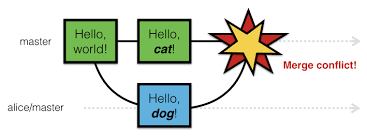
\includegraphics[scale=1]{mergeConflict.png}
\paragraph{}
In dieser Situation gibt es keine Möglichkeit die Änderungen zusammenzuführen, nun muss händisch untersucht werden, welche der Anderungen übernommen wird. Dies lässt sich nicht automatisch lösen, da nicht eindeutig ist welche der beiden Änderungen beibehalten werden kann.

\end{document}